\section{Background}
This section presents a review of existing algorithms, an anomaly taxonomy, and evaluation of existing anomaly detection libraries. Additionally, this section includes an overview of the Work Packages (WPs) that define the deliverables of the FIREMAN project.

\subsection{FIREMAN Work Packages}
\label{ref_FIREMAN_WP}

This subsection will outline the progress and overall goal of the three milestones or work packages that guide the FIREMAN project. The interconnection and overview of the individual WPs is shown in Figure \ref{fig:wp-diagram}

\begin{figure}[H]
    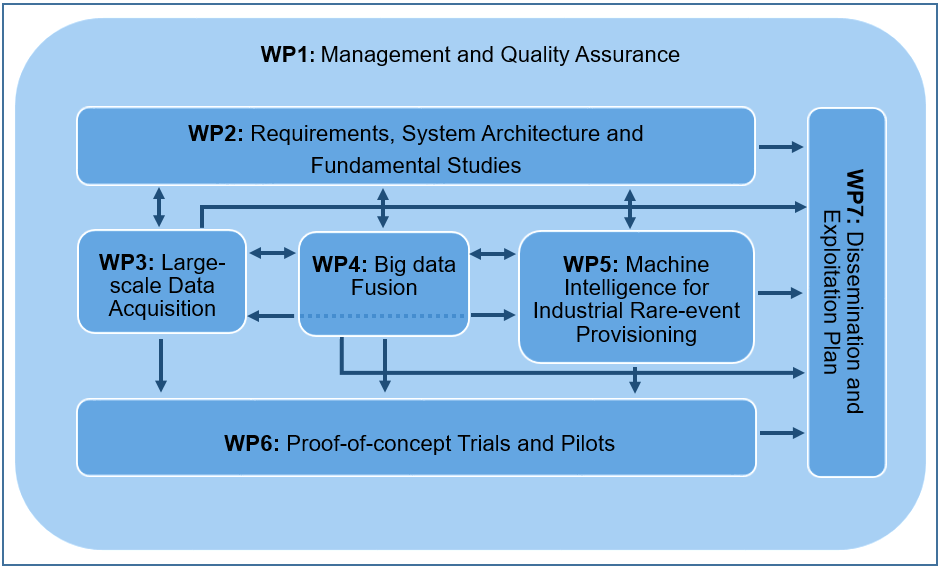
\includegraphics[width=0.8\textwidth]{Images/FIREMAN_pert_diagram.png}
    \caption{FIREMAN WP Diagram}
    \label{fig:wp-diagram}
\end{figure}

This work will focus on WP6 by demonstrating an implementation of a theoretical algorithm for real-world anomaly detection.

\subsubsection{Large Scale Data Acquisition (WP3)}

This work package focuses on \enquote{event-based modelling and traffic characterization techniques aiming for a reduced use of communication and storage resources. This pre-processing task is expected -among others- to optimize the subsequent data transmissions by injecting only relevant data in the network to reduce overhead and increase spectral efficiency.} \citel{wp3.1}

In this portion of FIREMAN, we examined a  variety of industrial data sets including the Tennessee Eastman Process, Electricity Metering, IEC-61850 Distribution Automation, and the EPFL Smart Grid Pilot. This data set is not heavily reliant on relational constraints or atomicity, consistency, isolation, durability (ACID) compliance. Because of this, we have selected a non-relational PostgreSQL database for storage because of its superior throughput and increased performance in data processing applications.

The developed detection framework for rare events is shown in Figure \ref{fig:three-layer}. The sensors traditionally used in Cyber-Physical Systems do not have much compute or storage capacity which makes pre-processing of data at the sensor level challenging. Because of this, \enquote{compression is essential for reducing the challenge of data storage, collection, transmission, processing, and analysis at the local level \parencite{compression}.} Authors \cite{wp3.2} have shown that it is possible to achieve a 92.6\% compression rate which means that only 7.4\% of samples are transmitted. We have also used different methods including linear interpolation to de-compress the data and have measured the error using the root mean square technique. 

\begin{figure}[H]
    % \centering
    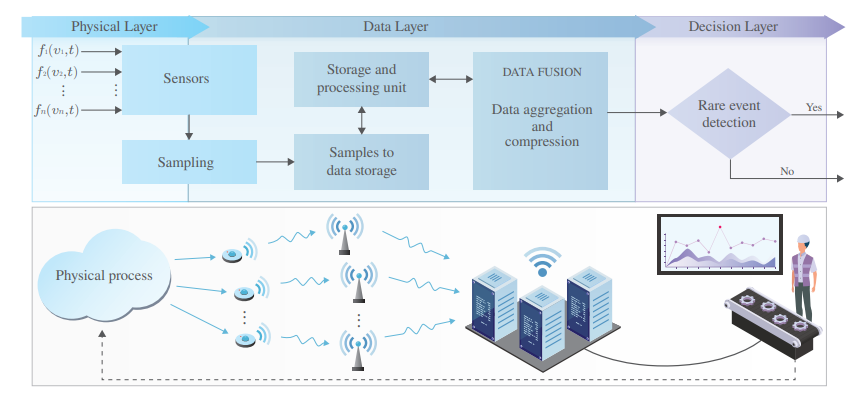
\includegraphics[width=0.8\textwidth]{Images/three-layer-system.PNG}
    \caption{Three layer framework for rare event detection \parencite{three-layer-approach}}
    \label{fig:three-layer}
\end{figure}

Modeling of transmission reduction techniques centered around the electricity modeling data set. Three approaches for reducing transmissions were presented including transmission on large spikes, transmissions on accumulated variance, and time interval defined transmission with a timeout to compensate for meter or network failure. These simulations have shown a large potential for reducing transmissions without significantly affecting the accuracy of the measured signal. We modeled a Markov-Modulated Poission Process to simulate these industrial processes for use in further stages of the project.

\subsubsection{Big Data Fusion (WP4)}
\label{ref_wp4}
The goal of this task is \enquote{to show how a large number of sensors and their corresponding data can be  accommodated and aggregated at small cost for reliably detecting rare events \parencite{wp4.1}.} This task focuses on three primary objects: 
\begin{inlinelist}
    \item heterogeneous data aggregation in machine-type communications;
    \item signature-based cluster formation; and
    \item IoT platform and database selection.
\end{inlinelist}

It is challenging to simultaneously connect a massive number of devices which is why data aggregation is important.
This strategy outlined by Authors \cite{massive-machine} relies on the following principals:
\begin{inlinelist}
  \item decreasing communication distance and power consumption of connected devices;
  \item utilizing an efficient distributed node routing network to decrease bandwidth congestion of central nodes; and
  \item extending the network coverage.
\end{inlinelist}
The researchers also introduced a cluster formation scheme based on signatures that reduces the signalling overhead required for peer-discovery in the network. This technique utilizes signal aggregates to reduce traffic congestion to the central node.

Additionally we surveyed IoT experts to determine the most important properties and components of an IoT system. This survey compared the five most popular cloud IoT providers: AWS, Azure, GCP, IBM Watson, and Oracle IoT to create a comparison that can be used by businesses when selecting a cloud provider that suits their business needs.

SEAT, an automotive component manufacturer, provided two use cases and accompanying data sets for the FIREMAN project. The first involves early failure detection of mechanical components in the drive chain in the Paint shop which causes axial displacement. The second involves detecting early failure of the spindle on a CNC machine which ensures lineal movement over a surface. In both of these situations detecting failure early will help SEAT detect problems and solve them before they begin to impact production components and eventually reduce production downtime to zero. 

\subsubsection{Machine Intelligence for Industrial Rare-event Provisioning (WP5)}

The goal of this task is to utilize machine intelligence techniques to predict indicators of health for a machine, component, or entire industrial process to determine health and detect premature failure. The main technique proposed in this task is Quantitative Association Rule Mining Algorithm (QARMA).

\enquote{QARMA is a family of algorithms for extracting all (or, depending on user inputs, an important subset of) valid non-dominated quantitative association rules that hold in a dataset, that can then be used for further data analysis such as deriving rule-based classifier ensembles or as explainers of classification results of other black-box classifiers.}\citel{wp5.1}  This technique is one of the most human understandable techniques for machine intelligence and has shown promise for this application. In this WP, QARMA is tested on the SEAT dataset discussed in \ref{ref_wp4}.

Traditional methods for pruning the rules created by the algorithm were analyzed in this WP as many of them can be extraneous or unreliable. The fastest open source Mixed-Integer Programming (MIP) tool was able to solve this problem in 19 seconds while the parallelized hybrid search algorithm proposed in this WP solved the problem 240 times faster when using parallel threads.

Authors \cite{wp5.1} used a breadth first search approach to compute a `small' subset of rules that cover the majority of instances in a training dataset covered by the totality of rules extracted by QARMA applied on it. Through experimentation on a synthetic power grid fault diagnostic dataset QARMA performs better than certain neural networks with noisy data. This is because of the over-fitting of training data with Deep Neural Network architectures. The rule based methods generated by QARMA produce human understandable rules which is beneficial in creating explainable AI.

\subsubsection{Proof-of-Concept Trails and Pilots (WP6)}
\label{ref_wp6}

% TODO

\subsection{Algorithm Explainability}

Certain high-risk use cases for machine learning algorithms demand a high level of explainability and confidence in the algorithm outputs to use in fields of decision making. In many cases an algorithm makes a classification decision but there is not a clear explanation as to why the algorithm made that decision. In the field of power electronics, understanding why a data-driven controller is making a decision is critical to incorporating it into real world power distribution scenarios. 

Answering these questions is complex and there are a few approaches to achieving this goal. Authors \cite{black-box-explainability} propose using conditional entropy to determine how each input is related to each output. The generated plots are then compared to the physical insights of the system and outlier, adversarial data that falls outside the plot is identified and removed. The model is then retrained. This technique is helpful for identifying and removing adversarial data that falls outside the range of accepted values but it would not identify data overloading in a specific portion of the graph which would create an incorrect classification.

\subsubsection{Model Uncertainty}
When analyzing uncertainty, it is important to distinguish between the two types discussed below.
\blockquote{
    \enquote{\textbf{Epistemic uncertainty} describes what the model does not know because training data was not appropriate. Epistemic uncertainty is due to limited data and knowledge. Given enough training samples, epistemic uncertainty will decrease. Epistemic uncertainty can arise in areas where there are fewer samples for training.
    
    \textbf{Aleatoric uncertainty} is the uncertainty arising from the natural stochasticity of observations. Aleatoric uncertainty cannot be reduced even when more data is provided. When it comes to measurement errors, we call it homoscedastic uncertainty because it is constant for all samples. Input data-dependent uncertainty is known as heteroscedastic uncertainty.}\citel{uncertainity-towards-data-science}
}

Aleatoric uncertainty describes phenomenon that arise inline with a given probability distribution. So if you have a signal that has noise inline with a given probability distribution, having more data on that signal will not change the noise probability distribution. Another way to think about it would be if you are at a train station recording audio and there will be 3 announcements that occur each hour that will disrupt your recording but you do not know when they will come. Having more data (hours) will not change the amount of announcements that occur. There are indeed some cases where having more data would reduce uncertainty but that is not what this property is discussing. It does not reference the data distribution itself but the distribution of random errors in the data.

With deep learning algorithms, it is important to know the level of confidence the model is predicting the outcome with. cite{explaining-adversarial-examples} explain that adding simple adversarial data (like small noise to a photo) will make an image recognition algorithm incorrectly classify one animal as a completely different one. This is further concerning since adversarial data does not need to be tailored to a specific algorithm. The transferability of this type of adversarial data allows it to be applied to many black box algorithms to achieve an unintended or potentially malicious result. 

A malfunctioning sensor or bad connection can generate noise (a type of aleatoric uncertainty), which cannot be fixed by more measurements or more data. Data imputation can be used as a technique to correct for or understand this type of uncertainty. If you can identify that the uncertainty is present, then you can use data imputation to form a well educated guess as to what the value should actually be. The significance of identifying it as aleatoric uncertainty is that no amount of model tuning or data collection can fix the underlying issue, so data imputation presents an opportunity to move forward that standard techniques would not.

Bayseaian techniques can be used to create a probability distribution over the weights to determine a level of uncertainty for the weights. Unfortunately, retraining a large number of models on a variety of data sets is computationally expensive and time consuming. Authors \cite{gal2016dropout} proposed using a dropout technique to approximate the Bayseaian representation. This technique avoids over-fitting by randomly sampling and dropping network nodes across many different training iterations.

It is important to perform the dropout technique while training and testing the algorithm and then compute the variance to determine the uncertainty. This enables researchers to determine that for specific values the algorithm is providing a best guess answer with high levels of uncertainty, which could then signal the need for human intervention or review in decision making.  

\subsection{Outlier Taxonomy}

The term `outlier' or `anomaly' can have a variety of interpretations and meanings depending on the context. In order to select and evaluate appropriate techniques for outlier detection, it is essential to understand and define the various types of outliers that can be present in a dataset. There are conventionally three ways that outliers are categorized in literature visualized graphically in figure \ref{fig:outliers-graphic} and described below:
\blockquote{
\textbf{Point outliers} are singular data points that are anomalous in the context of the entire dataset or window. \enquote{The extreme values could lead to serious consequences, and therefore point outliers are often the focus of sequential outlier detection research.}\parencite{lai2021revisiting} These outliers can be non-temporal or temporal in nature and often represent phenomenon like intermittent sensor failure. 

\textbf{Contextual outliers}  \enquote{are the individual instances that are anomalous under a specific context, such as
the discord points within the same harmonic pattern. Contextual outliers usually have relatively
larger/smaller values in their own context but not globally.}\parencite{lai2021revisiting}

\textbf{Collective outliers} are \enquote{defined as a collection of related data instances that are anomalous with respect
to the entire data set. Specifically, the individual points of a collective outlier may not be anomalous
by themselves but the co-occurrence of them becomes an outlier. Collective outliers are ubiquitous
in sequential data since there are often strong dependencies among time points.}\parencite{lai2021revisiting}
}

\begin{figure}[H]
    % \centering
    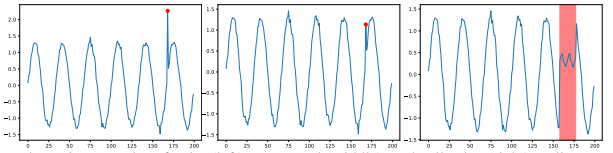
\includegraphics[width=0.8\textwidth]{Images/outliers_graphic.PNG}
    \caption{\enquote{Point (left), Contextual (middle), and Collective (right) outliers} \parencite{lai2021revisiting}}
    \label{fig:outliers-graphic}
\end{figure}

It is useful in analyzing data to be more specific with the phenomenon discussed and the type of outlier detection desired. As such, the taxonomy of outliers will be outlined in the following sections for this work \parencite{lai2021revisiting}.

\subsubsection{Point-wise Outliers}
Point-wise outliers can fall into 2 categories: global and contextual.
\begin{itemize}
    \item \textbf{Global point outliers} are individual points significantly outside the overall distribution in the context of the entire dataset.
    \item \textbf{Contextual point outliers} are individual points significantly outside the overall distribution in the context of a specific window or subset of the dataset. (ex. during tea-time when everyone is using electricity).
\end{itemize} 
\subsubsection{Pattern-wise Outliers}
Pattern-wise outliers can fall into 3 categories: shaplet, seasonal, and trend outliers. Figure \ref{fig:contextual-outliers} shows these phenomenon visually. This subset of anomalies represents various anomalous sub-sequences of the data in a given context. 
\begin{itemize}
    \item \textbf{Shaplet outliers} are one or a series of subsequences that has a dissimilar basic shaplet (pattern) compared with the standard data shaplet (pattern).
    \item \textbf{Seasonal outliers} represent seasonal abnormalities. Seasonality is the overall pattern of the data during a given time-span. Detecting abnormalities in seasonality often represents unusual phenomenon (ex. a spike in web traffic due to a holiday, or an increase in residential power demand because to a major televised sporting event). 
    \item \textbf{Trend outliers} are abnormal subsequenes that resultingly alter the overal distribution of the following data. This is the type of outlier that is present in one of the data sets analyzed in this work and will be a focus of the detection strategies presented. 
\end{itemize} 

\begin{figure}[H]
    % \centering
    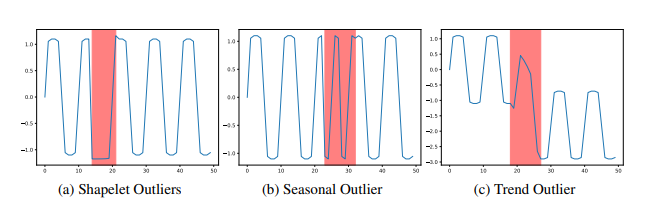
\includegraphics[width=0.8\textwidth]{Images/contextual_outliers_graphic.PNG}
    \caption{Three types of Pattern-wise Outliers \parencite{lai2021revisiting}}
    \label{fig:contextual-outliers}
\end{figure}

\subsection{Anomaly Detection Algorithms}
\label{ref_anomaly_detection_alg}

Numerous outlier detection techniques currently exist each is traditionally applied to one domain specific problem. These techniques are very versatile (especially unsupervised ones) and as such can be applied in a much more general sense. This section will focus on current developments and advances across all disciplines in anomaly detection techniques.

While there are many new and state-of-the-art developments, corresponding code to a publication is often not included. This makes reproducing the results presented in the paper difficult and in order to utilize these techniques in practice, the algorithm has to be implemented based on pseudo-code, a time consuming process. As such, this will serve primarily as a survey of promising techniques. Section \ref{ref_code_libraries} examines existing implementations of some of these algorithms.

\subsubsection{Streaming Half Space Trees (HST)}
\enquote{Streaming Half-Space Trees (HST) are a fast one-class anomaly detector for evolving data streams.}\parencite{fast-anomaly-detection-streaming} It is an efficient method for point-wise outlier detection and is implemented in a variety of anomaly detection libraries. This technique relies on ensembleing HS-Trees which are full binary trees, where all leaves are at the same depth. It is fast, relatively efficient with a time and space complexity of $O(1)$, and is suitable for handling streaming data.

% \subsubsection{RS Hash}

% \subsubsection{Isolation Forests}

\subsubsection{Local Outlier Factor (LOF)}

The Local Outlier Factor (LOF) technique assigns a degree of `outlierness' to each datapoint as opposed to a binary classifier. The traditional LOF method is used to detect outliers in static datasets. Since it must compute neighborhood distances for each data point, which must be recomputed entirely when a new datapoint is added, it is not well suited for streaming data. Many researchers including \parencite{dilof-data-streams}, \parencite{fast-memory-efficent-lof-milof} have proposed streaming adaptations to the base LOF algorithm. The extensions modify the algorithm to be suitable for stream learning as well as improve memory and computational performance and speed. This algorithm is well suited to point-wise contextual outlier detection.

\subsubsection{Matrix Profile} % TODO: improve matrix profile section
\label{ref_matrix-profile-alg}
\enquote{The Matrix Profile is a vector that represents the distances between all subsequences within a time seires and their nearest neighbors.} \parencite{yeh2016matrix-profile-1} The matrix profile technique has a variety of advantages including speed and generalizability to a variety of problem domains. 

\enquote{The Matrix Profile computes a distance profile and profile index. The distance profile is a vector of minimum Z-Normalized Euclidean Distances. The profile index holds the position of the closest neighbor which represents the most similar sub-sequence. The algorithms that compute the Matrix Profile use a sliding window approach. With a window size of m, the algorithm}\parencite{matrix-profile-intro}:
\begin{enumerate}
    \item \enquote{Computes the distances for the windowed sub-sequence against the entire time series
    \item Sets an exclusion zone to ignore trivial matches
    \item Updates the distance profile with the minimal values
    \item Sets the first nearest-neighbor index}\parencite{matrix-profile-intro}
\end{enumerate}

Using this technique, it is easy to extract information from the data. Motifs which are repeated patterns or discords which are anomalies can both be discovered in a dataset with the Matrix Profile technique. 

% \subsubsection{LSTM}

% \subsubsection{One-Class SVM}

% \subsubsection{Vector Autoregressor}

% \subsubsection{STL}

% \subsubsection{Clustering}

% \subsubsection{Deep Neural Network (DNN)}

% \subsubsection{Inlier Priority of Discriminate Network}

% \subsubsection{Set-Based Processing}

\subsection{Anomaly Detection Libraries}
\label{ref_code_libraries}
 Libraries and algorithms were surveyed from a variety of Github repositories, online sources, and a comprehensive framework list from Author \cite{medico2020-ts-list}. The most relevant libraries were selected and their performance is evaluated against the sample data sets in Section \ref{ref_results}. The following criteria was required for a framework to be selected for analysis:
 \begin{inlinelist}
     \item written for Python
     \item compatibility with MacOS, Windows, and Linux operating systems
     \item actively maintained with git commits within the past two years
     \item suitable for context-wise anomaly detection on signals
     \item quality documentation
     \item over 100 stars on Github.
 \end{inlinelist}
 
 
Some libraries were excluded from selection because their focus on production environments makes them difficult to test and perform research with. In further research these libraries may be considered to implement a production outlier detection pipeline. Many of them use the underlying algorithms described in Section \ref{ref_anomaly_detection_alg} for detection. 
 
Table \ref{tab:anom_detect_lib} compares the selected outlier detection libraries in a systematic way. This table can be used to quickly compare and evaluate libraries for use in implementation. The specific algorithms for each library are classified into a category with a description.
 
Each method is classified according to how suitable it is for online learning and its primary use case. For the algorithm to have a yes in the online learning category, the algorithm must be able to iteratively update the model efficiently, and predict specific instance one at a time. Partially in the online category means that there is a pre-trained model, with individual instance detection. No in the online category means that the algorithm is not suited for online detection. 

\bigskip
\begin{longtable}{llllp{2.75cm}}
\caption{Outlier Detection Overview [(\textbf{PA}): Point-wise Anomaly, (\textbf{CA}): Context-wise Anomaly, (\textbf{DD}): Drift Detection, (\textbf{S}): Segmentation)]}\\
\toprule
\textbf{Library} & \textbf{Algorithm} & \textbf{Focus} & \textbf{Online} & \textbf{Description} \\
\midrule
\endfirsthead
\multicolumn{5}{c}%
{\tablename\ \thetable\ -- \textit{Continued from previous page}} \\
\hline
\textbf{Library} & \textbf{Algorithm} & \textbf{Focus} & \textbf{Online} & \textbf{Description} \\
\hline
\endhead
\hline \multicolumn{5}{r}{\textit{Continued on next page}} \\
\endfoot
\bottomrule
\endlastfoot
    PySAD\footcite{pysad} & Indivdidual Models &  \textbf{PA} & yes & Score anomalies \\
    & Probability Calibrators & \textbf{S} & yes & Convert raw scores to probabilities\\
    \midrule 
    PyOD\footcite{zhao2019pyod} & Individual Models &  \textbf{PA} & no & Score anomalies\\
    \midrule 
    River\footcite{2020river} & Individual Models &  \textbf{PA} & yes & Score anomalies\\
    & Drift models & \textbf{DD} & yes & Detect concept drift \\
    & Time-series models & \textbf{S} & yes & Segment time-series data \\
    \midrule
    STUMPY\footcite{law2019stumpy} & Matrix Profile \footcite{yeh2016matrix-profile-1} &  \textbf{CA} & yes & Time-series subsequence analysis\\
    & Time Series Chains\footcite{Zhu2017-time-series-chains} & \textbf{CA, DD} & no  & Motif drift detection \\
    & FLUSS \& FLOSS\footcite{2017-fluss-floss} & \textbf{CA, S} & yes & Time-series segmentation\\
    \midrule 
    tsod\footcite{tsod} & Simple Detectors &  \textbf{CA, PA} & partial & Gradient and range detectors \\
    \midrule 
    TODS\footcite{Lai_2021_TODS} & Detection Algorithms &  \textbf{CA, PA} & partial & Detect anomalies\\
    & Feature Analysis & \textbf{S} & partial & Statistics based segmentation\\
    \midrule 
    Alibi Detect\footcite{alibi-detect} & Outlier Detection & \textbf{CA, PA} & partial & Anomaly detection\\
    & Adversarial Detection & \textbf{CA} & partial & Detect adversarial data \\
    & Drift Detection & \textbf{DD} & partial & Concept drift identifications \\
    \midrule 
    banpei\footcite{banpei} & Hotelling's Theory &  \textbf{PA} & yes & Outlier detection\\
    & SST & \textbf{S} & yes & Change point detection \\
    \midrule 
    SaxPy\footcite{senin2018grammarviz-saxpy} & SAX &  \textbf{PA, S} & no & Symbolic Aggregate approXimation \\
    & EMMA & \textbf{CA, S} & no & Time-series motif discovery\\
    \midrule 
    Darts\footcite{herzen2021darts} & Filtering Models & \textbf{CA} & no & Gaussian, Kalman, Moving Average Filter \\
    & Forecasting Models & \textbf{S} & no & Predictive forecasting \\
    \midrule 
    Merlion\footcite{bhatnagar2021merlion} & Anomaly Algorithms &  \textbf{CA, PA} & yes & Anomaly Detection strategies \\
    & Forecasting & \textbf{S} & yes & Predictive forecasting \\
    \midrule 
    Luminaire\footcite{chakraborty2020building-luminaire} & Structural Modeling &  \textbf{ PA } & yes & Anomaly detection \\
    & Windowed Density Model & \textbf{CA, DD} & yes & Anomalous window detection using KL divergence \\
    \label{tab:anom_detect_lib}
\end{longtable}



\subsubsection{PySAD}

\enquote{PySAD is an open-source python framework for anomaly detection on streaming multivariate data.} \parencite{pysad} PySAD can operate in a streaming context so models can be updated as new data points arrive. This is both computational and memory efficient. PySAD also provides a variety of pre-processing, post-processing, and probability calculation tools. This library provides both univariate and multivariate prediction models for supervised and unsupervised data. 

\subsubsection{PyOD}

\enquote{PyOD is a python framework for anomaly detection on non-streaming data. PySAD provides an interface for PyOD for certain batch processing tasks. PyOD includes more than 30 detection algorithms.} \parencite{zhao2019pyod} Its features include:
 \begin{itemize}
     \item \enquote{Unified APIs, detailed documentation, and interactive examples across various algorithms.
     \item Advanced models, including classical ones from scikit-learn, latest deep learning methods, and emerging algorithms like COPOD.
     \item Optimized performance with JIT and parallelization when possible, using numba and joblib.}\parencite{zhao2019pyod}
 \end{itemize}

\subsubsection{River}

River is a streaming machine learning library that provides tools for anomaly detection, drift detection, and more. It is a fast and efficient library that can learn and predict with single instances. Some of its features include:
 \begin{itemize}
     \item \enquote{Linear models with a wide array of optimizers
     \item Nearest neighbors, decision trees, naïve Bayes
     \item Anomaly detection
     \item Time series forecasting
     \item Imbalanced learning}\parencite{2020river}
 \end{itemize}


\subsubsection{STUMPY}
STUMPY is a library used to compute the uni-variate or multi-variate matrix profile for provided time series data created by U.S. based investment firm TD Ameritrade. In its simplest form, the algorithm compares element-wise distances between each sub-sequence for each point, known as a self-similarity join. This naive method is very computationally expensive with a complexity of $O(n^2m)$. STUMPY introduces a computationally efficient way to compute the matrix profile defined in Section \ref{ref_matrix-profile-alg}. The library incorporates various gpu-accelerated methods to further improve performance. \enquote{This can be used for a variety of time series data mining tasks including}\parencite{law2019stumpy}: 
\begin{itemize}
    \item \enquote{pattern/motif (approximately repeated subsequences within a longer time series) discovery
    \item anomaly/novelty (discord) discovery
    \item shapelet discovery
    \item semantic segmentation
    \item streaming (on-line) data
    \item fast approximate matrix profiles
    \item time series chains (temporally ordered set of subsequence patterns)
    \item snippets for summarizing long time series
    \item pan matrix profiles for selecting the best subsequence window size(s)}\parencite{law2019stumpy}
\end{itemize}
STUMPY is well suited to analyzing pattern-wise outliers in the dataset and finding anomalies, called discords in this discipline. This library will be used to create and analyze a uni-variate and multi-variate Matrix Profile for the sample dataset. 

\subsubsection{tsod}

The tsod package aims to provide examples and algorithms for detecting anomalies in time series data specifically tailored to the water domain \parencite{tsod}. Although it is designed for the water domain, the techniques can be analyzed and used in a variety of other domains. It includes a gradient detection technique for detecting abrupt changes that will be explored.

\subsubsection{TODS}
\enquote{TODS provides a varity of automated machine learning tools for outlier detection on multivariate time-series data. It includes many state-of-the-art algorithms and anomaly detection techniques.}\parencite{Lai_2021_TODS}. It strengths are in the following areas:
\begin{itemize}
    \item \textbf{Full Stack Machine Learning System} with support for prepossessing, feature extraction, detection algorithms, and human-in-the-loop interfaces.
    \item \textbf{Extensive Algorithms}, including PyOD's point-wise detection algorithms, pattern-wise detection algorithms, and ensemble algorithms for global anomaly detection.
    \item \textbf{Automated Machine Learning} to provide knowledge-free processes that construct optimal pipelines based on the provided data by automatically searching for the best combination of techniques from existing modules.
\end{itemize}

\subsubsection{Alibi Detect}
Alibi Detect is a library developed by U.K. based Seldon for outlier, adversarial, and drift data detection compatible with TensorFlow and PyTorch backends \parencite{alibi-detect}. There are a variety of supported algorithms for these three types of data detection tasks and the package is actively maintained. The company also provide and maintain an enterprise machine learning deployment platform that integrates with Alibi Detect. The researchers will explore this further in subsequent work when examining the production pipeline. The framework handles streaming and offline data detection for time series, tabular, text, and image data. 

\subsubsection{banpei}

\enquote{Banpei is a Python package of the anomaly detection}\parencite{banpei}. It implements the Singular spectrum transformation (SST) algorithm for change point detection and Hotelling's theory for outlier detection. It was designed to offer real time monitoring functionality and operates on streaming data.

\subsubsection{SaxPy}

Symbolic Aggregate approximation (SAX) is used to transform a series of numerical data points into a sequence of letters \parencite{senin2018grammarviz-saxpy}. The library implements HOT-SAX, a time series anomaly detection algorithm. 

% \subsubsection{RNN-Time-Series}

\subsubsection{Darts}
Darts is python machine learning package developed by the Swiss AI company Unit8 for time series data forecasting. The library provides a variety of advanced and classic models with a sci-kit learn compatible interface. \enquote{The emphasis of the library is on offering modern machine learning functionalities such as supporting multidimensional series, meta-learning on multiple series, training on large datasets, incorporating external data, ensembling models, and providing a rich support for probabilistic forecasting.} \citel{herzen2021darts}

\subsubsection{SalesForce's Merlion}
\enquote{Merlion is a Python library for time series intelligence. It provides an end-to-end machine learning framework that includes loading and transforming data, building and training models, post-processing model outputs, and evaluating model performance. It supports various time series learning tasks, including forecasting and anomaly detection for both univariate and multivariate time series.}\citel{bhatnagar2021merlion} 
The differentiating factors of the library are:
\begin{itemize}
    \item \enquote{Standardized and easily extensible data loading \& benchmarking for a wide range of forecasting and anomaly detection datasets.
    \item A library of diverse models for both anomaly detection and forecasting, unified under a shared interface. Models include classic statistical methods, tree ensembles, and deep learning approaches. Advanced users may fully configure each model as desired.
    \item AutoML for automated hyperaparameter tuning and model selection.
    \item Practical, industry-inspired post-processing rules for anomaly detectors that make anomaly scores more interpretable, while also reducing the number of false positives.
    \item Flexible evaluation pipelines that simulate the live deployment \& re-training of a model in production, and evaluate performance on both forecasting and anomaly detection.}\citel{bhatnagar2021merlion}
\end{itemize}

\subsubsection{Zillow's Luminaire}

\enquote{Luminaire is a python package that provides ML-driven solutions for monitoring time series data. Luminaire provides several anomaly detection and forecasting capabilities that incorporate correlational and seasonal patterns as well as uncontrollable variations in the data over time.}\citel{chakraborty2020building-luminaire} This library provides a technique to monitor data points over a window of time which is helpful in detecting context-wise outliers in a streaming context.






